\section{Diagnostics và forecast uncertainty}

\subsection{Residual diagnostics}

Diagnostics được thực hiện trên recovered latent demand proxy. Với target là tổng 7 ngày tiếp theo, các forecast origin liên tiếp có target window overlap mạnh: forecast tại ngày $t$ và ngày $t+1$ chia sẻ 6/7 ngày trong target. Vì vậy, residual rolling evaluation có thể còn autocorrelation một phần do thiết kế target, không nhất thiết chỉ do model thiếu pattern.


\begin{table}[H]
\centering
\caption{Diagnostics trên recovered latent demand proxy}
\label{tab:long-diagnostics}
\resizebox{\linewidth}{!}{%
\begin{tabular}{llllllllll}
\toprule
Model & RMSE & MAE & WAPE & WPE & Residual mean & Residual std & Ljung-Box p-value & Jarque-Bera p-value & N \\
\midrule
Recovered naive x7 & 4.3949 & 2.8080 & 0.3149 & -0.0198 & 0.1770 & 4.3913 & 0.1790 & 0.0000 & 70000 \\
Recovered seasonal naive 7-day & 2.9113 & 1.7704 & 0.1985 & -0.0614 & 0.5475 & 2.8594 & 0.0131 & 0.0000 & 70000 \\
Recovered rolling mean 14-day & 3.1099 & 1.8367 & 0.2060 & -0.0807 & 0.7194 & 3.0255 & 0.0001 & 0.0000 & 70000 \\
Observed-sales forecasting & 3.6749 & 2.1780 & 0.2442 & -0.1788 & 1.5943 & 3.3111 & 0.0127 & 0.0000 & 70000 \\
Recovered-demand forecasting & 3.6160 & 1.8082 & 0.2028 & -0.0800 & 0.7134 & 3.5450 & 0.0665 & 0.0000 & 70000 \\
Recovered seasonal-ML hybrid & 3.2106 & 1.7545 & 0.1967 & -0.0726 & 0.6470 & 3.1448 & 0.0311 & 0.0000 & 70000 \\
\bottomrule
\end{tabular}
}
\end{table}



\begin{figure}[H]
    \centering
    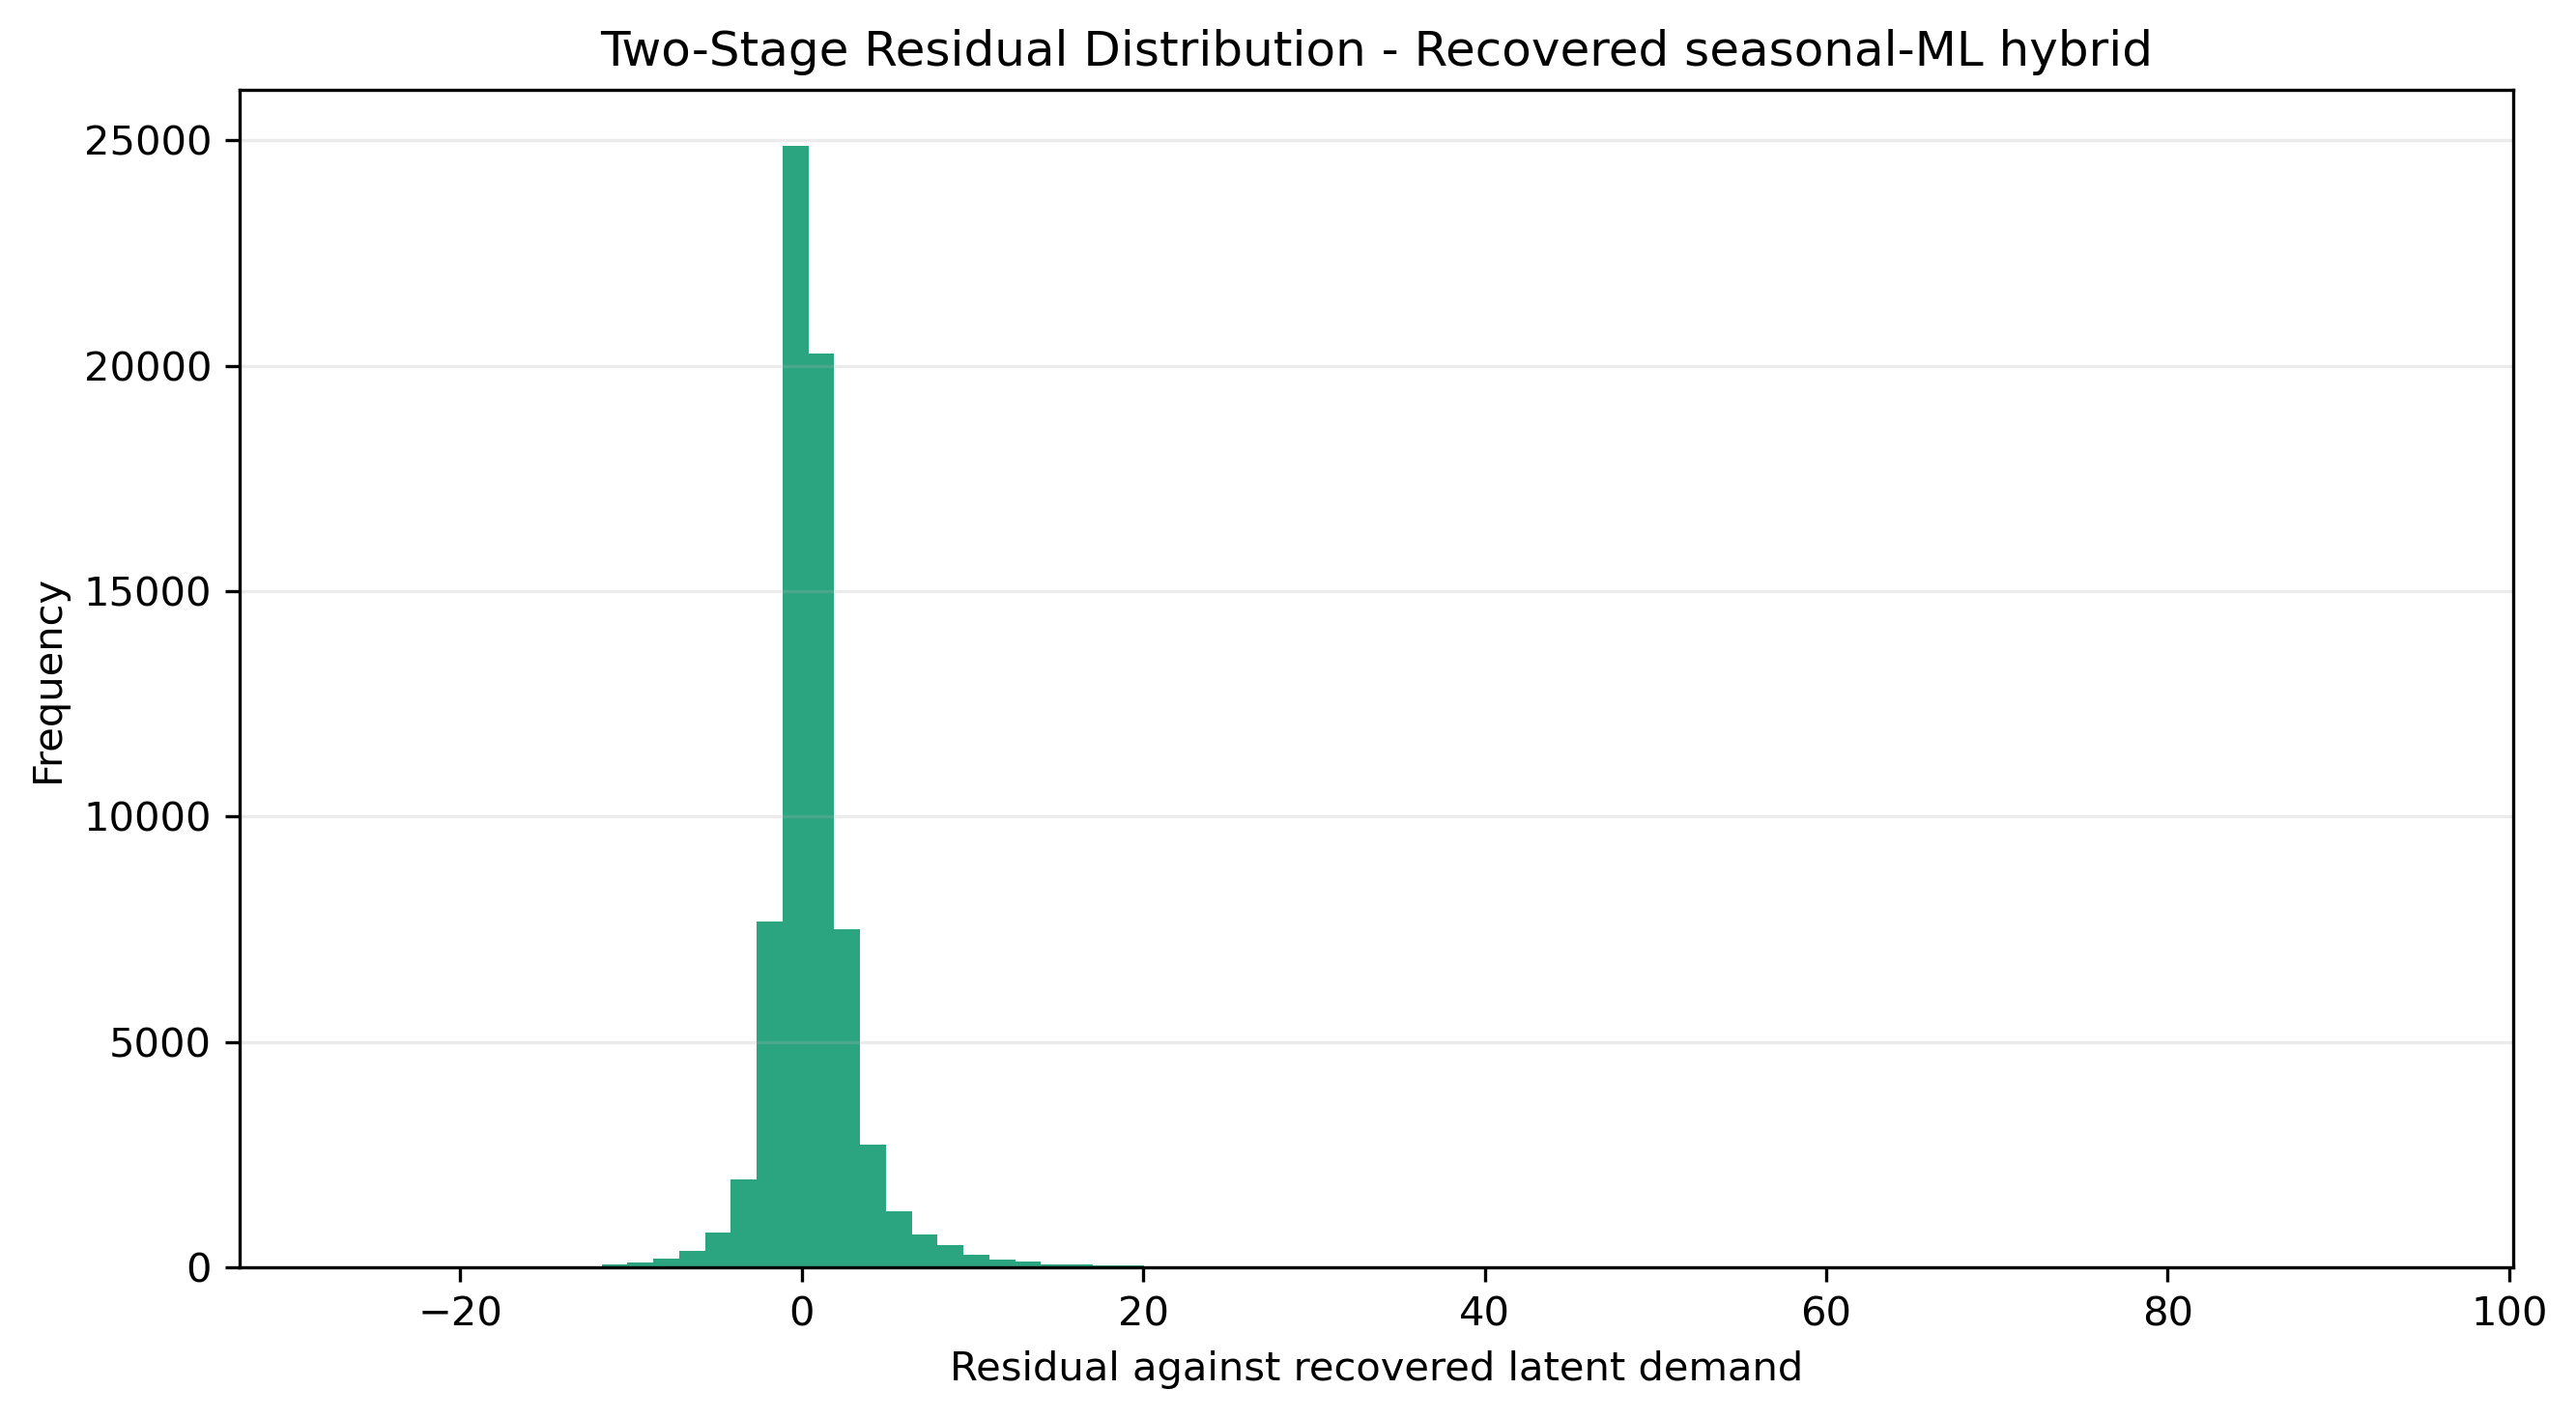
\includegraphics[width=0.78\linewidth]{figures/owner_two_stage_residual_distribution.png}
    \caption{Phân phối residual của mô hình chính.}
    \label{fig:long-residual-dist}
\end{figure}



\begin{figure}[H]
    \centering
    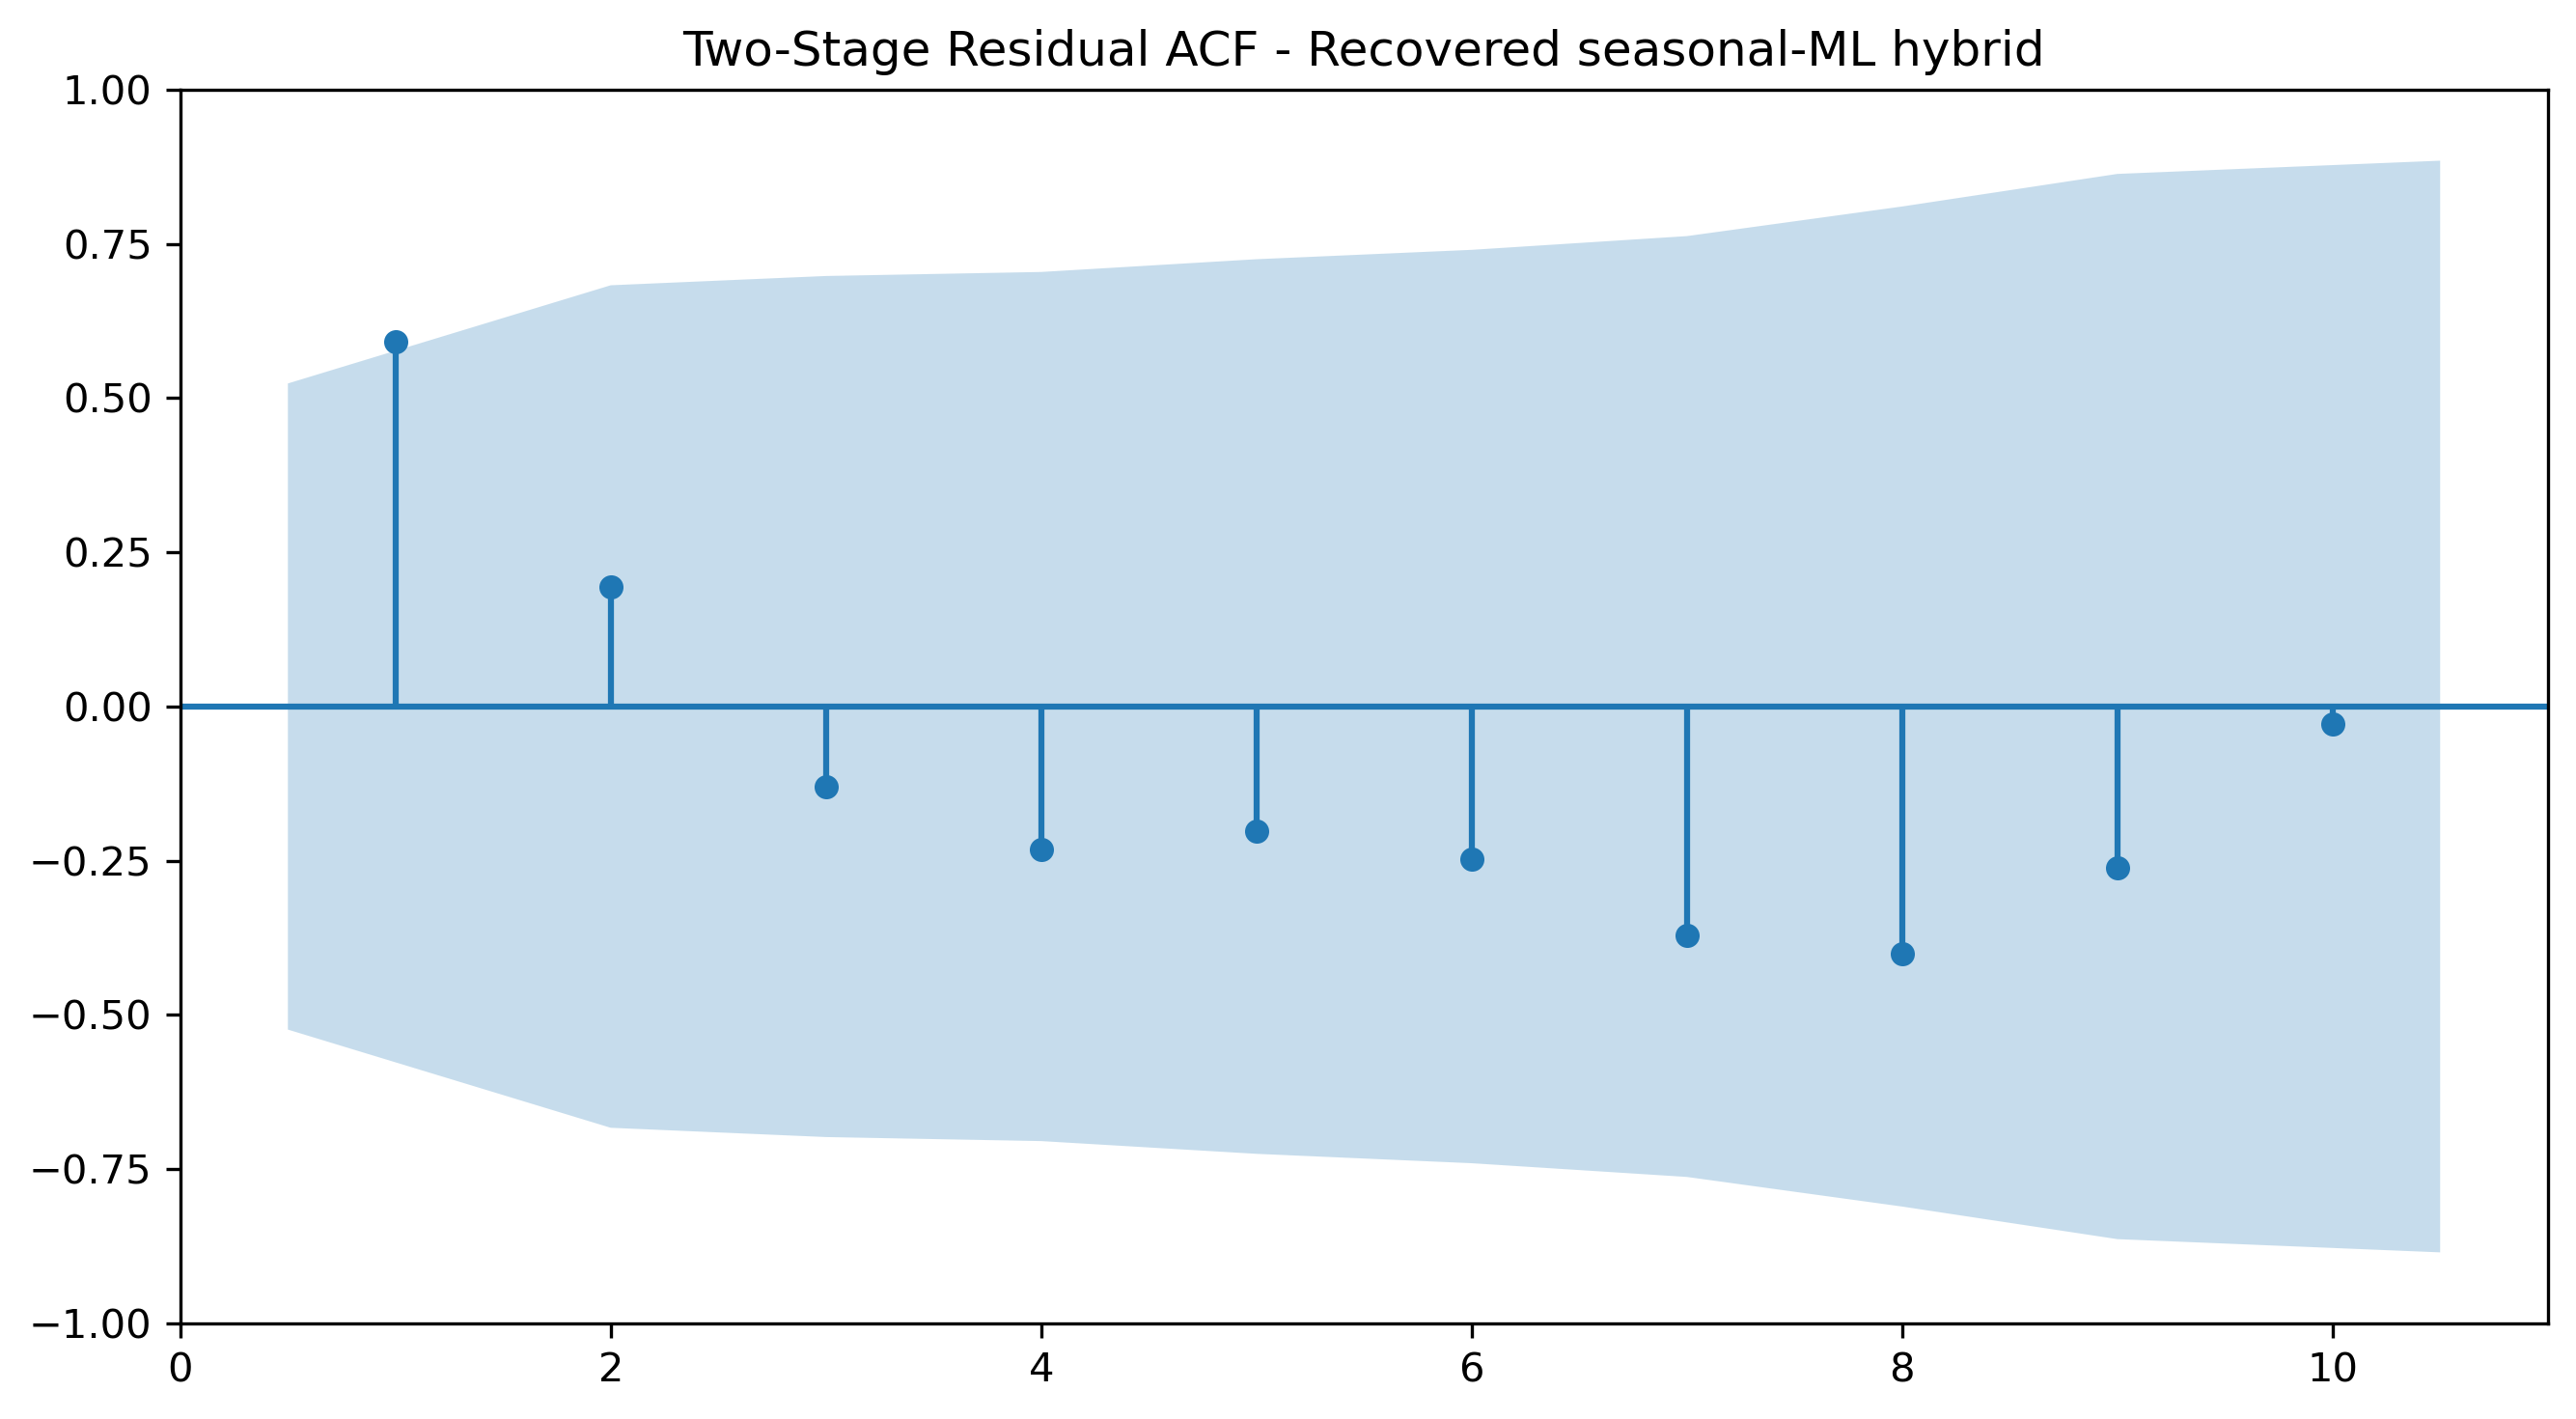
\includegraphics[width=0.82\linewidth]{figures/owner_two_stage_residual_acf.png}
    \caption{Residual ACF của mô hình chính.}
    \label{fig:long-residual-acf}
\end{figure}


\subsection{Non-overlap diagnostics}

Báo cáo bổ sung non-overlap diagnostics bằng cách lấy forecast origin cách nhau 7 ngày. Kiểm tra này công bằng hơn với target next-7-day, nhưng test window chỉ có 14 ngày nên chỉ có rất ít aggregate points. Vì vậy, đây là sanity check phụ, không phải bằng chứng tuyệt đối rằng residual độc lập hoàn toàn.


\begin{table}[H]
\centering
\caption{Diagnostics trên non-overlapping 7-day targets}
\label{tab:long-nonoverlap}
\resizebox{\linewidth}{!}{%
\begin{tabular}{lllllllll}
\toprule
Model & Evaluation dates & RMSE & MAE & WAPE & WPE & Ljung-Box p-value & N & Aggregate residual points \\
\midrule
Recovered naive x7 & 2024-06-11; 2024-06-18 & 4.6707 & 2.9483 & 0.3389 & 0.0080 & 0.1573 & 10000 & 2 \\
Recovered seasonal naive 7-day & 2024-06-11; 2024-06-18 & 2.8150 & 1.7140 & 0.1970 & -0.0662 & 0.1573 & 10000 & 2 \\
Recovered rolling mean 14-day & 2024-06-11; 2024-06-18 & 3.0150 & 1.7821 & 0.2049 & -0.0738 & 0.1573 & 10000 & 2 \\
Observed-sales forecasting & 2024-06-11; 2024-06-18 & 3.5320 & 2.1044 & 0.2419 & -0.1753 & 0.1573 & 10000 & 2 \\
Recovered-demand forecasting & 2024-06-11; 2024-06-18 & 3.3906 & 1.7544 & 0.2017 & -0.0716 & 0.1573 & 10000 & 2 \\
Recovered seasonal-ML hybrid & 2024-06-11; 2024-06-18 & 3.0564 & 1.7001 & 0.1954 & -0.0695 & 0.1573 & 10000 & 2 \\
\bottomrule
\end{tabular}
}
\end{table}


\subsection{Prediction intervals}

Khoảng dự báo được xây dựng từ phân vị residual validation. Cách này không giả định residual chuẩn tuyệt đối, phù hợp hơn với dữ liệu bán lẻ thưa và nhiều spike.


\begin{figure}[H]
    \centering
    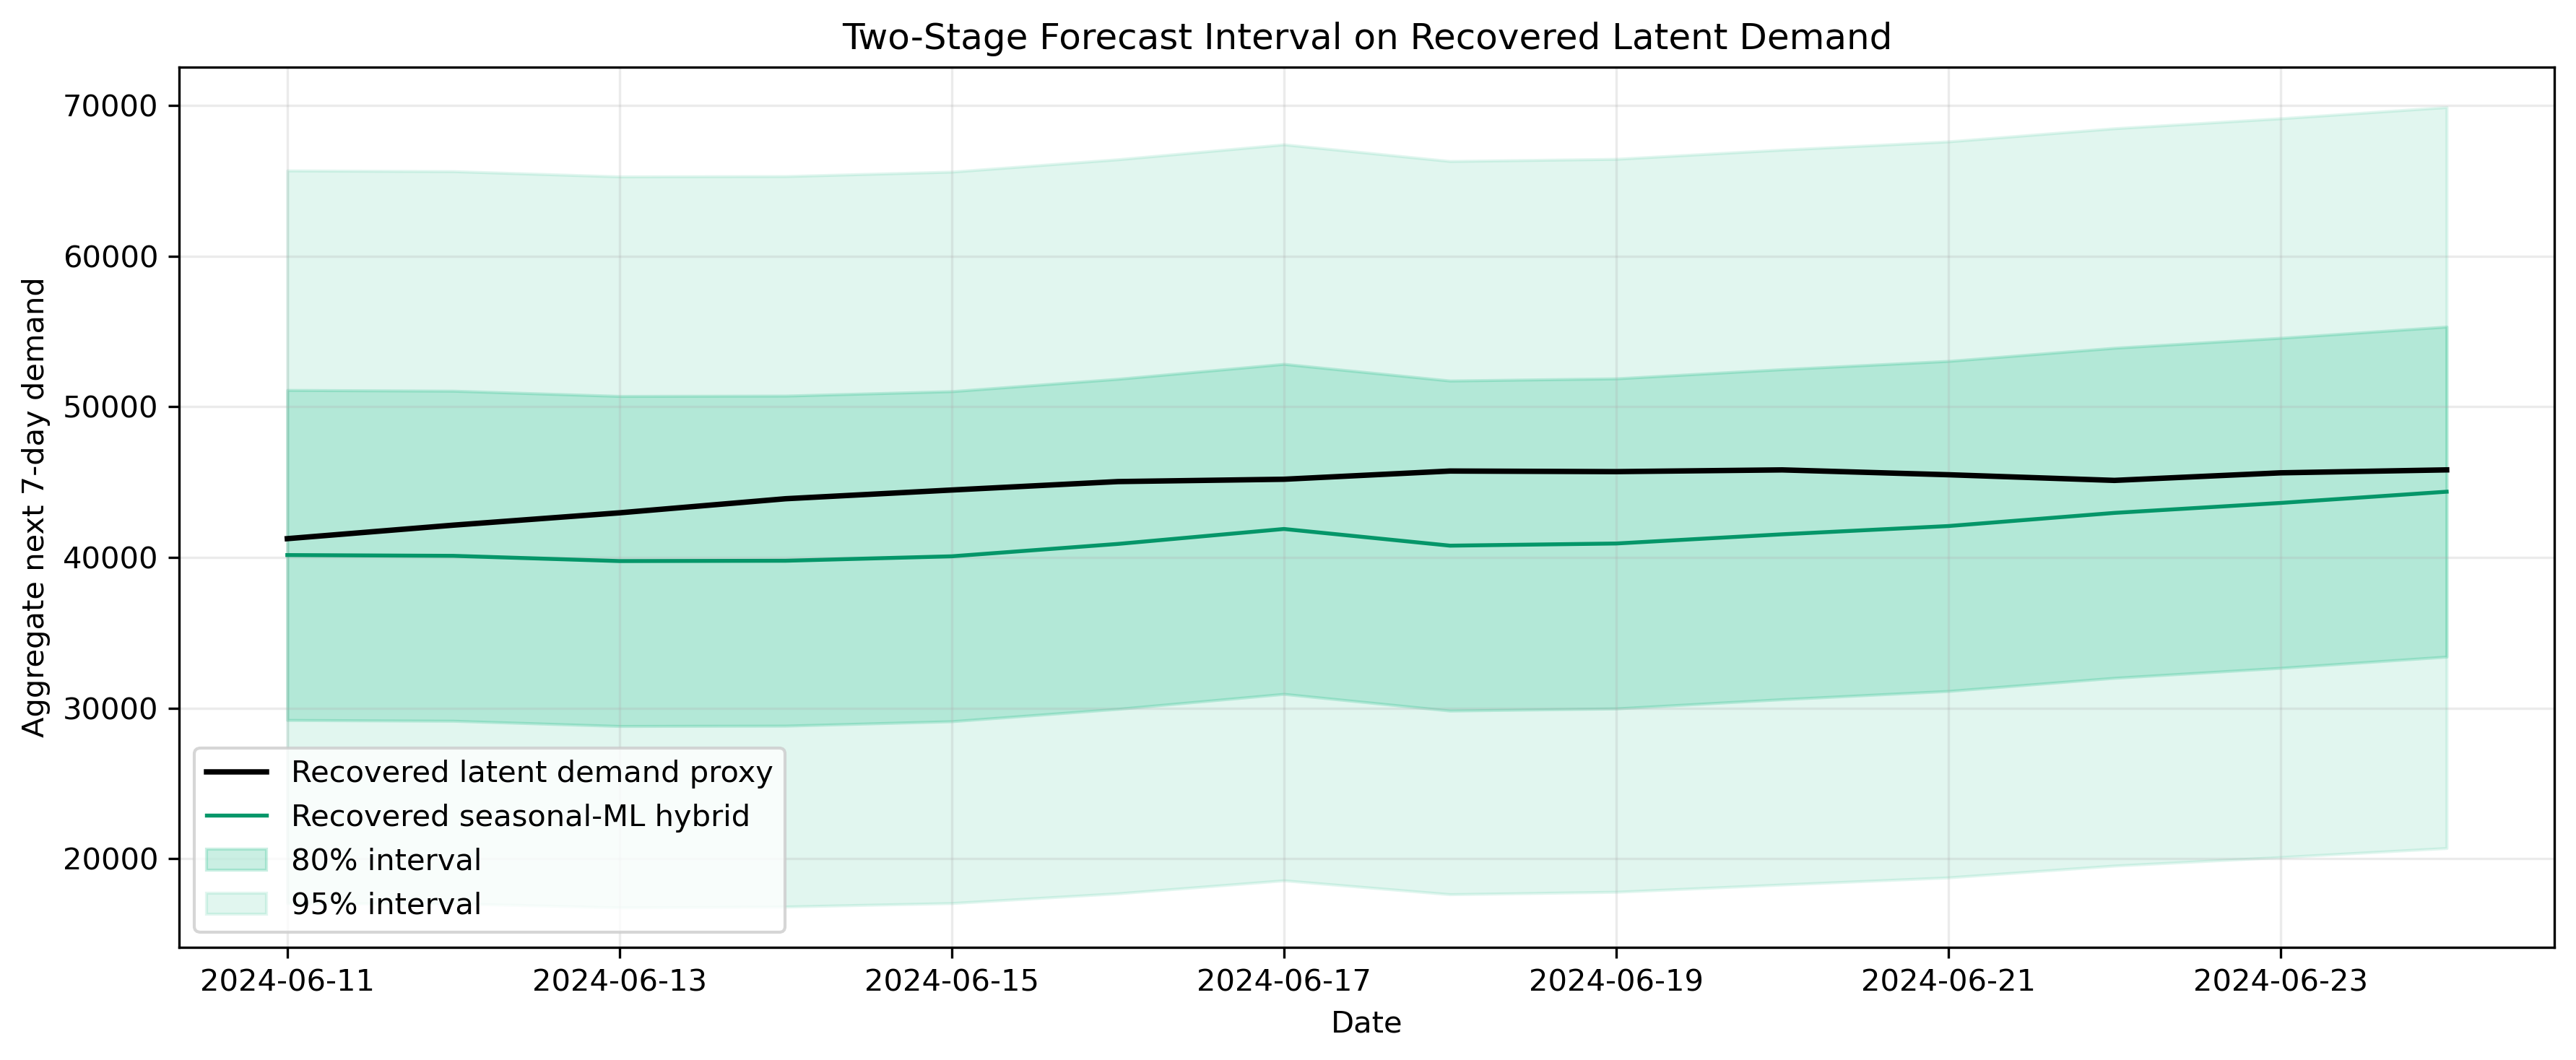
\includegraphics[width=0.92\linewidth]{figures/owner_two_stage_forecast_interval.png}
    \caption{Khoảng dự báo 80\textbackslash\{\}\% và 95\textbackslash\{\}\% cho mô hình chính.}
    \label{fig:long-forecast-interval}
\end{figure}
